% CS6140 Homework Assignment Template
% Computer Science
% Northeastern University
% Boston, MA 02115

% Do not manipulate any of the settings
\documentclass[twoside]{article}

\usepackage{epsfig}
\usepackage{natbib}
\usepackage{units}
\usepackage{amssymb}
\usepackage{amsmath}
\usepackage{babel}


\setlength{\oddsidemargin}{0 in}
\setlength{\evensidemargin}{0 in}
\setlength{\topmargin}{-0.6 in}
\setlength{\textwidth}{6.5 in}
\setlength{\textheight}{8.5 in}
\setlength{\headsep}{0.75 in}
\setlength{\parindent}{0 in}
\setlength{\parskip}{0.1 in}

\newcommand{\lecture}[3]{
   \pagestyle{myheadings}
   \thispagestyle{plain}
   \newpage
   \setcounter{page}{1}
   \noindent
   \begin{center}
   \framebox{
      \vbox{\vspace{2mm}
    \hbox to 6.28in { {\bf CS6140: Machine Learning\hfill} }
       \vspace{6mm}
       \hbox to 6.28in { {\Large \hfill #1  \hfill} }
       \vspace{6mm}
       \hbox to 6.28in { {\it Assigned: #2 \hfill Due: #3} }
      \vspace{2mm}}
   }
   \end{center}
   \markboth{#1}{#1}
   \vspace*{4mm}
}

\begin{document}

% to have alphanumeric enumeration (Hasan's command)
\renewcommand{\labelenumi}{\alph{enumi})}

\lecture{Homework Assignment \# 3}{02/11/2020}{03/03/2020, 11:59pm, through Blackboard}

\begin{center}
Submitted By: Piyush Goel (goel.pi@husky.neu.edu)
\end{center}


\begin{enumerate}
\item \textbf{Project title} - Predicting the clinical impact of human mutation with deep neural networks
\item Names of the team members and their Northeastern University emails.\\
Piyush Goel - goel.pi@husky.neu.edu
\item \textbf{Objectives and significance}
     \begin{enumerate}
     \item The \textbf{goal} of the project is to reproduce and verify the paper - Sundaram, L., Gao, H., Padigepati, S.R. et al. Predicting the clinical impact of human mutation with deep neural networks. (Ref. a)
     \item \textbf{Significance}: While most genetic mutations are benign, some have deleterious effects on health. If we could classify mutations as benign or harmful, then we could possibly use it to our advantage in making medicine, or preventing disease before it even starts to show any symptoms, the possibilities are be endless.
     \item The \textbf{motivation} for doing this project is to reproduce the paper, verify the results, and learn in the process. Also, this problem seems like one which could have a huge positive impact on human health and lives in general, in the foreseeable future.
     \end{enumerate}
\item \textbf{Background}\\
	 Genetics (Ref. b):
     \begin{enumerate}
     \item DNA, or deoxyribonucleic acid, is the hereditary material in humans and almost all other organisms. Nearly every cell in a person’s body has the same DNA. The information in DNA is stored as a code made up of four chemical bases: adenine (A), guanine (G), cytosine (C), and thymine (T). Human DNA consists of about 3 billion bases, and more than 99 percent of those bases are the same in all people. The order, or sequence, of these bases determines the information available for building and maintaining an organism. A set of 3 of these bases is called a codon and each codon corresponds to one of twenty possible Amino Acids.
     \item The human body has 23 pairs of chromosomes and each chromosome is made up of multiple genes. A gene is the basic physical and functional unit of heredity. Genes are made up of DNA. 
     \item A gene mutation is a permanent alteration in the DNA sequence that makes up a gene, such that the sequence differs from what is found in most people. Mutations range in size; they can affect anywhere from a single DNA building block (base pair) to a large segment of a chromosome that includes multiple genes.
     \item Most disease-causing gene mutations are uncommon in the general population. However, other genetic changes occur more frequently. Genetic alterations that occur in more than 1 percent of the population are called polymorphisms. They are common enough to be considered a normal variation in the DNA. Polymorphisms are responsible for many of the normal differences between people such as eye color, hair color, and blood type. Although many polymorphisms have no negative effects on a person’s health, some of these variations may influence the risk of developing certain disorders.
     \item Some genes act as instructions to make molecules called proteins. To function correctly, each cell depends on thousands of proteins to do their jobs in the right places at the right times. Sometimes, gene mutations prevent one or more of these proteins from working properly. By changing a gene’s instructions for making a protein, a mutation can cause the protein to malfunction or to be missing entirely. When a mutation alters a protein that plays a critical role in the body, it can disrupt normal development or cause a medical condition. A condition caused by mutations in one or more genes is called a genetic disorder. In some cases, gene mutations are so severe that they prevent an embryo from surviving until birth.
     \item Only a small percentage of mutations cause genetic disorders—most have no impact on health or development. For example, some mutations alter a gene's DNA sequence but do not change the function of the protein made by the gene. A very small percentage of all mutations actually have a positive effect.
     \item Because a person's genetic code can have a large number of mutations with no effect on health, diagnosing genetic conditions can be difficult. Sometimes, genes thought to be related to a particular genetic condition have mutations, but whether these changes are involved in development of the condition has not been determined; these genetic changes are known as variants of unknown significance (VOUS) or (VUS). Sometimes, no mutations are found in suspected disease-related genes, but mutations are found in other genes whose relationship to a particular genetic condition is unknown. It is difficult to know whether these variants are involved in the disease.
     \end{enumerate}
 	 Deep Learning:
 	 \begin{enumerate}
 	 \item Deep Learning is a type of machine learning method which simply uses neural networks with multiple hidden layers to learn the input to output mapping function.
 	 \item Convolutional Neural Networks are a class of Deep Neural Networks which are primarily applied to vision based tasks. A Convolutional Layer consists of a kernel which when convoluted with the input produces the output of the layer. 
 	 \item The Convolutional Layers, are generally applied to image type of data, but can also be applied to 1-D data like text or genetic sequence using a single dimensional kernel.
 	 \item Batch normalization is a technique for improving the speed, performance, and stability of artificial neural networks. It is used to normalize the input layer by adjusting and scaling the activations.
 	 \item Sometimes the output of a layer is sent to not just the next layer but also to a layer further down the path, i.e. skipping a few layers, this is called a skip connection.
 	 \item Activation functions are applied to the outputs of the neural network layer to introduce non-linearity in the network which helps it learn complex functions. ReLU (Rectified Linear Unit) is one such very widely used activation function. Its equation is $f(x) = max\{0, x\}$. The sigmod function is another activation function which is generally applied to the last layer of the neural network to make binary classifications. Its equation is $f(x) = \frac{1}{1 + e^{-x}}$
 	 \end{enumerate}
  	 Uniqueness:
  	 \begin{enumerate}
  	 \item This paper tries to classifies mutations by training on gene mutation data not only from humans but also from the primates genetically close to humans since most of the mutations are extremely rare in humans and hence are rarely observed, this provides a way to collect large enough data to train a deep neural network. It also has a good accuracy.
     \end{enumerate}
\pagebreak
\item \textbf{Proposed approach}\\

	 Method and Implementation:
	 \begin{enumerate}
	 \item Deep Neural Networks will be used, constituting mainly 1-D Convolutional Layers with Batch Normalization and the ReLU activation function. The output layer would be using the Sigmoid activation function instead of ReLU, and then one Global Max-pooling Layer (which simply outputs the maximum) as well. The network contains some skip connections as well.
	 \item The output of the network is the pathogenicity score for the given mutation.
	 \item the model takes multiple matrices as input for one mutation:
	 \begin{enumerate}
	 	\item A 51 length reference amino acid sequence, i.e. the sequence before the mutation, centered at the point where the mutation will occur.
	 	\item A 51 length alternate amino acid sequence, i.e. the sequence after the mutation, centered at the point where the mutation occurred.
	 	\item A 51 length position weight matrix calculated using the data from 11 primates.
	 	\item A 51 length position weight matrix calculated using the data from 50 mammals excluding primates.
	 	\item A 51 length position weight matrix calculated using the data from 38 vertebrates.
	 	\item Output of a pretrained solvent accessibility prediction network which takes as input the position weight matrix calculated using the data from all 99 vertebrates.
	 	\item Output of a pretrained secondary structure prediction network which takes as input the position weight matrix calculated using the data from all 99 vertebrates.
  	 \end{enumerate}
   	 \item Since there are 20 different possible Amino Acids, therefore each of the 51 length matrix would be 51x20 instead, since either one-hot encoding or the position weight matrix are used.
   	 \item Python 3 will be used to do most of the coding, and some minor shell scripting to manipulate or look through the data (since the data files are extremely large and can not be loaded into the ram whole at once). The major third-party python libraries required are Tensorflow, Keras, Pandas and Numpy, more may be included if necessary.
   	 \item The model architecture to be implemented is on page 5.
   	 \item The architecture for the solvent accessibility and secondary structure prediction models is the same and is on page 6.
	 \end{enumerate}

	 Data:
     \begin{enumerate}     
     \item The genetic sequences for GRCh37/hg19 (homo-sapiens) are obtained from the Genome Aggregation Database (gnomAD) (Ref. e), and through the REST API provided by UCSC Genome Browser (Ref. c) to access the data as required. The authors of the paper also provided some data which contains all of the mutations which they used for training and testing.
     \item The actual neural network which predicts the probability of a mutation being pathogenic requires the outputs of two previously trained neural networks which determine a protein's (a sequence of amino acids) secondary structure and solvent accessibility. The plan is to use these weights for now. But if time permits and retraining of these networks is tried then data from the Protein Data Bank (Ref. f) would be required.
     \end{enumerate}
\pagebreak
 	 Evaluation Strategy:
 	 \begin{enumerate}
 	 	\item The classification accuracy would be used to determine if the model works as intended.
 	 \end{enumerate}
  
  	 Expected Outcomes:
  	 \begin{enumerate}
  	 	\item The accuracy of model on both withheld common primate variants and clinical variants increases with the number of benign variants used to train the network.
  	 	\item Training on variants from each of the six non-human primate species independently contributes to an increase in the performance of the network, whereas training on variants from more distant mammals negatively impacts the performance of the network.
  	 \end{enumerate}
   
   	 Fallback Option:
   	 \begin{enumerate}
   	 	\item In case the initial idea fails, the input to the model could be modified to use only the reference and alternate amino acids. This would significantly simplify the network, and even eliminating the need for the secondary structure and solvent accessibility prediction networks. But this would also very likely result in reduced accuracy, since now the network will have lesser information about the amino acid sequence, for example it would now have no idea about its secondary structure.
   	 \end{enumerate}

\item \textbf{Individual tasks}
     \begin{enumerate}
     \item There is only one team member so all of the work will be done by one person.
     \end{enumerate}

\item \textbf{References}
     \begin{enumerate}
     \item https://www.nature.com/articles/s41588-018-0167-z
     \item https://ghr.nlm.nih.gov/primer
     \item http://genome.ucsc.edu/
     \item https://en.wikipedia.org/
     \item https://gnomad.broadinstitute.org/
     \item https://www.rcsb.org/
     \end{enumerate}
\end{enumerate}
\newpage

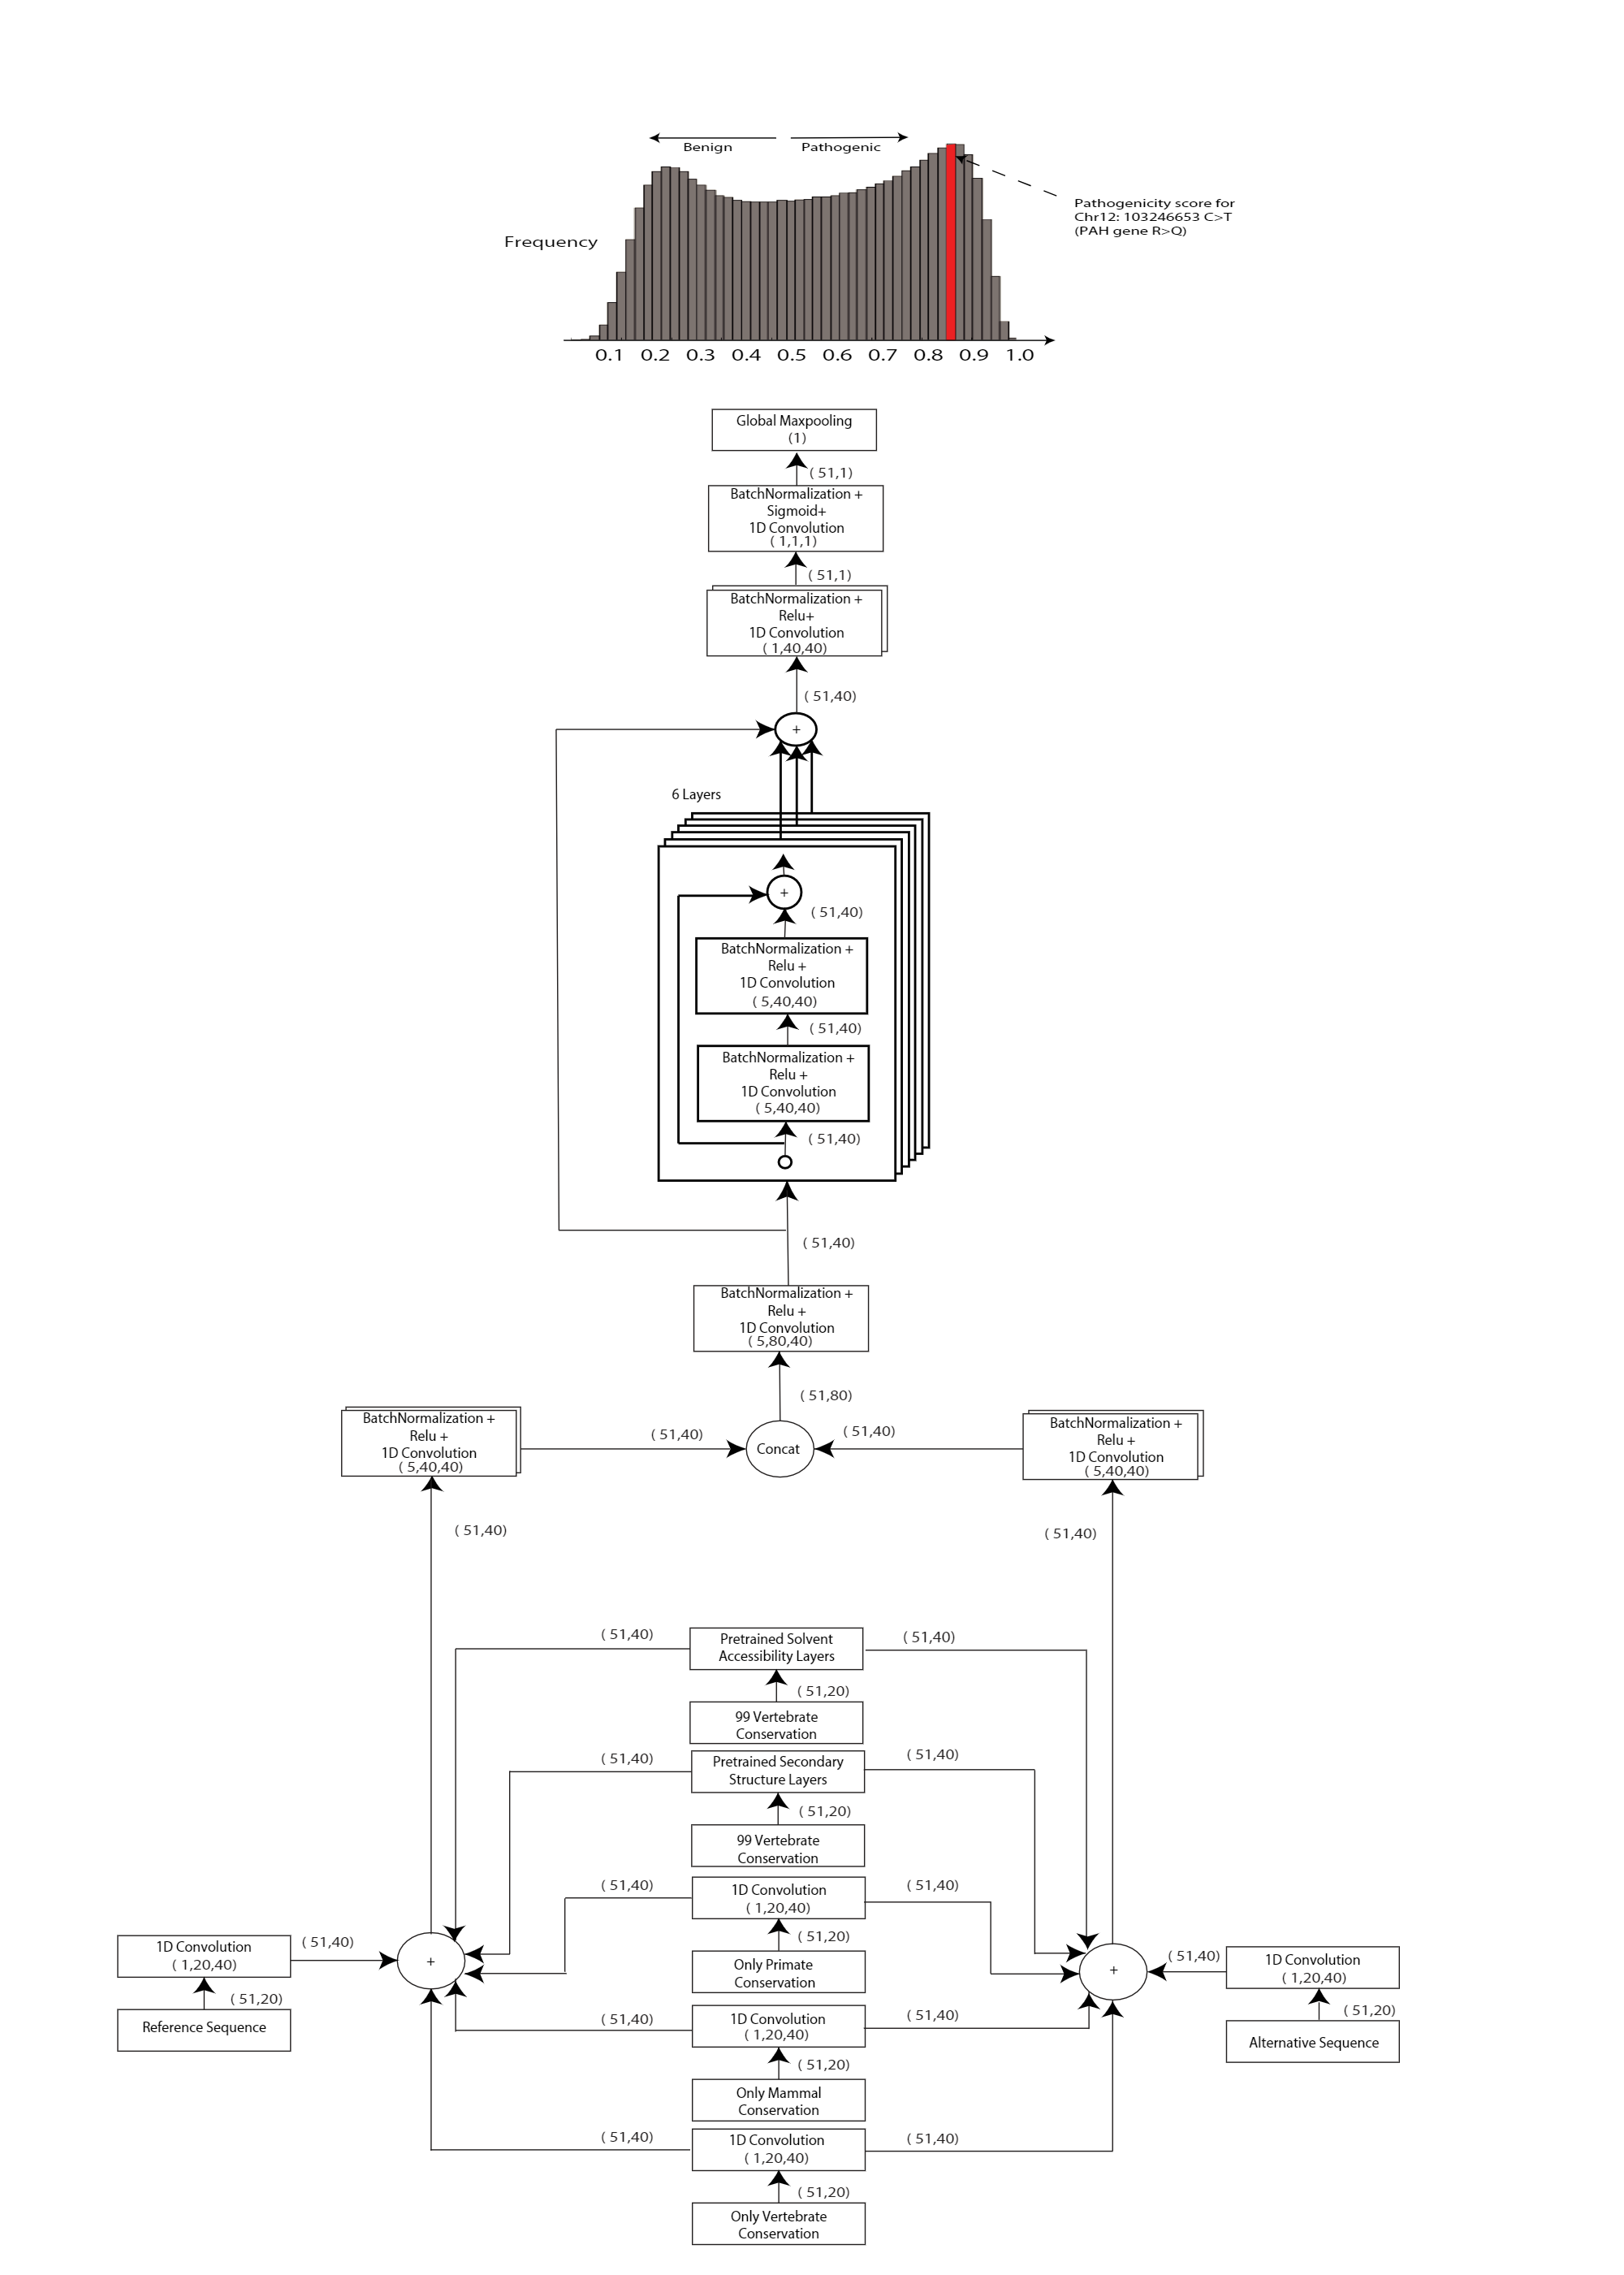
\includegraphics[scale=0.22]{Model}\\
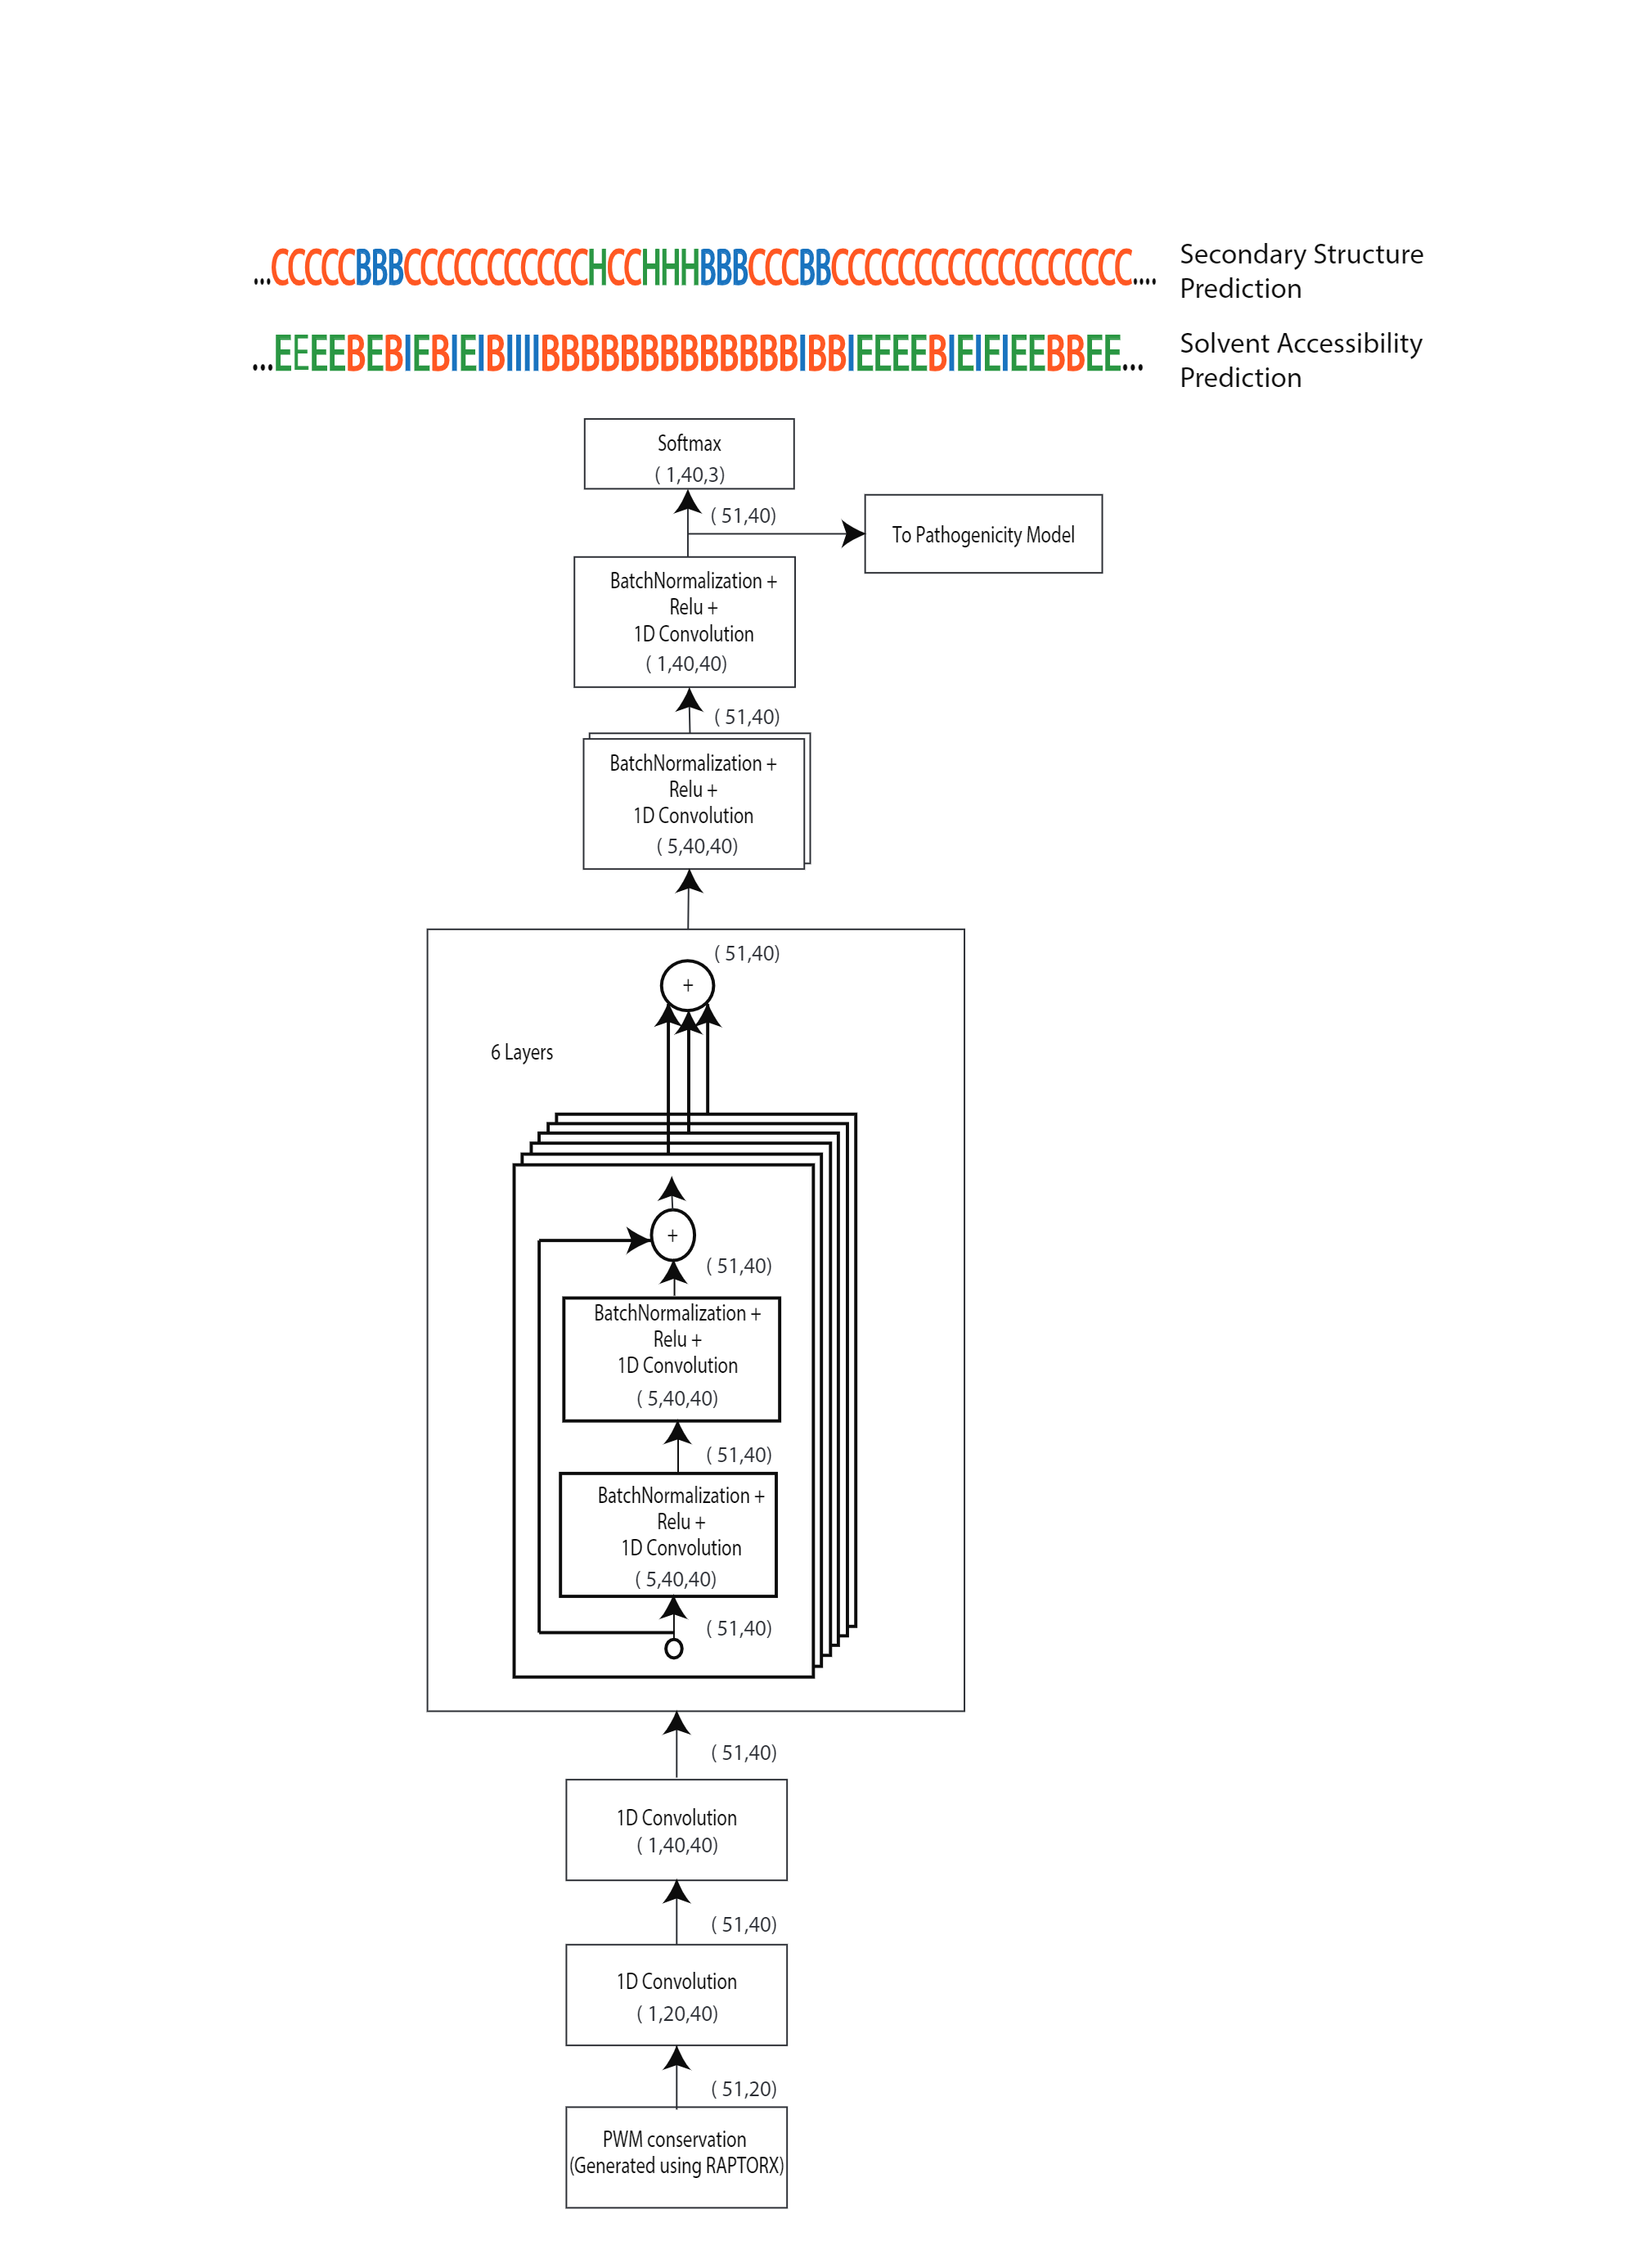
\includegraphics[scale=0.24]{Model2}

\end{document}
